\documentclass{beamer}

\usetheme{CambridgeUS}
\usefonttheme[onlylarge]{structurebold}
\setbeamerfont*{frametitle}{size=\normalsize,series=\bfseries}
\setbeamertemplate{navigation symbols}{}

\usepackage{kotex}
\usepackage{listings}

\definecolor{codegreen}{rgb}{0,0.6,0}
\definecolor{codegray}{rgb}{0.3,0.3,0.3}
\definecolor{backcolour}{rgb}{0.95,0.95,0.92}
\definecolor{purple}{rgb}{0.5, 0.0, 0.5}

\newcommand\Fontvi{\fontsize{8}{9.6}\selectfont}

\begin{document}

\lstset {
	language=java, 
	backgroundcolor=\color{backcolour},   
	commentstyle=\color{codegreen},
    keywordstyle=\color{purple},
	tabsize=4,
	showspaces=false, 
	showstringspaces=false,   
	breaklines=true
}

\title{안드로이드 컴포넌트의 이해}
\author[노재춘]{\texttt{suribada@gmail.com}}
\date[\today]{네이버 지도지역서비스개발랩}

\begin{frame}
\titlepage
\end{frame}

\begin{frame}
SQLite DB Lock 문제는 왜 발생하고, 해결 방법은 무엇인가?
\end{frame}

\setbeamercovered{transparent=20}
\begin{frame}
\frametitle{SQLite 기본}
\begin{itemize}
\item 시퀄라이트인가? 에스큐엘라이트냐?
\item Thread에서 쿼리를 실행하는 것이 좋은가?
\end{itemize}
\end{frame}

\begin{frame}
\frametitle{군더더기 코드들}
\begin{itemize}
\item 쿼리를 실행하는 메소드마다 synchronized를 해놓는다.
\item 단순 쿼리조차도 DB Transaction을 해놓는다.
\end{itemize}
\end{frame}

\begin{frame}
\frametitle{문제들}
\begin{itemize}
\item android.database.sqlite.SQLiteDatabaseLockedException이 발생하지만 원인을 알 수 없고, 재현이 잘 안 된다.
\item 왜 사용자들은 crash가 많을까?
\item 타이밍 이슈는 언제나 힘들다.
\end{itemize}
\end{frame}

\begin{frame}
\frametitle{Lock 기본 내용}
\begin{itemize}
\item 읽기 할 때는 Shared Lock을 잡는다. 다른 Shared Lock과 공존할 수 있다.
\item 쓰기 할 때는 Exclusive Lock을 잡는다. 다른 Lock을 허용하지 않는다.
\end{itemize}
\end{frame}

\begin{frame}
\frametitle{Lock의 상태 5가지(1)}
\begin{itemize}
\item UNLOCKED: 기본상태로 읽기나 쓰기가 안 된다.
\item SHARED: 읽기만 되고 쓰기는 안 된다. 동시에 여러 개의 프로세스가 Shared Lock을 가질 수 있다. 하나 이상의  Shared Lock이 활성화 되어 있다면, 다른 프로세스에서 쓰기를 할 수 없다. 쓰기를 위해서는 Shared Lock이 모두 해제될 때까지 대기한다.
\item RESERVED: 프로세스가 미래 어느 시점에 쓰기를 하려고 한다는 일종의 Flag Lock이다. Reserved Lock은 한번에 하나의 Reserved Lock만 있을 수 있으며, 여러 개의 Shared Lock과 공존할 수 있다. Reserved Lock 상태에서는 새로운 Shared Lock을 더 잡을 수도 있다.
\end{itemize}
\end{frame}

\begin{frame}
\frametitle{Lock의 상태 5가지(2)}
\begin{itemize}
\item PENDING: 가능한한 빨리 Lock을 잡고 있는 프로세스가 쓰기를 하려고 한다. 즉, 현재의 모든 Shared Lock이 clear되면서 Exclusive Lock을 가지려 한다. Pending Lock 상태에서는 이미 존재하는 Shared Lock은 허용되지만, 새로운 Shared Lock을 잡을 수는 없다. 
\item EXCLUSIVE: 파일에 쓰기 위해서 필요하다. 오직 하나의 Exclusive Lock만 허용되고, 다른 Lock은 공존할 수 없다. SQLite에서는 동시성을 높이기 위해서 Exclusive Lock을 잡는 시간을 최소화하려 하는데, 우리가 만드는 코드 내에서도 Exclusive Lock 구간을 줄이도록 노력해야 한다.
\end{itemize}
\end{frame}

\begin{frame}
\frametitle{Lock 문제 재현}
\begin{itemize}
\item https://github.com/touchlab/Android-Database-Locking-Collisions-Example
\item 에러가 발생해야 하는데 안 날 수도 있다. 이 때는 스레드 갯수를 늘려보면 반드시 발생시킬 수 있다.
\end{itemize}
\end{frame}

\begin{frame}
\frametitle{Lock 문제 재현을 통한 결론}
\begin{itemize}
\item 여러 스레드에서 별도의 SQLiteDatabase 인스턴스를 가지고 있으면 읽기와 쓰기가 함께 있는 경우 Lock 에러를 발생시킨다.
\item 반대로, 여러 스레드에서도 오직 하나의 SQLiteDatabase 인스턴스 만을 가지고 명령을 실행한다면, Lock  에러는 발생하지 않는다.
\end{itemize}
\end{frame}

\begin{frame}
\frametitle{왜 그럴까?}
\begin{itemize}
\item 안드로이드에서 SQLite의 default threading mode가 serialized이기 때문이다. 즉 명령어들은 순차적으로 실행된다.
\item threading mode 관련한 내용은 SQLite 사이트를 참고하자. http://www.sqlite.org/threadsafe.html
\end{itemize}
\end{frame}

\begin{frame}
\frametitle{하나의 인스턴스만?}
\begin{itemize}
\item SQLiteDatabase 인스턴스를 하나만 가지고서 serialized mode로 동작한다면 속도가 느려지진 않을까? 결론적으로 그렇다.\\
쓰기와 읽기가 함께 있는 것이라면 serialized mode가 되어야만 Lock 문제가 없기 때문에 하나의 인스턴스를 사용해야 하지만, 읽기만 있다면 굳이 하나의 인스턴스를 고집할 필요가 없다.
\end{itemize}
\end{frame}

\begin{frame}
DB Lock과 Transaction은 왜 한 묶음으로 얘기하는 것일까?
\end{frame}

\begin{frame}
\frametitle{DB Lock과 Transaction}
\begin{itemize}
\item 일반적인 CUD에서는 Lock을 잡아봐야 아주 짧은 시간이기 때문에 큰 영향을 주지는 않는다. 가장 Lock을 오래 잡을 수 있는 케이스로는 쓰기를 한꺼번에 해야 하는 Transaction이다.
\end{itemize}
\end{frame}

\begin{frame}
\frametitle{Transaction 사용하기}
\begin{itemize}
\item 필요한 경우에는 가능하면 쓰는 것이 좋다. \\
ex) 여러 데이터를 한꺼번에 입력하기
\item 케이스마다 다르지만, 실행 속도가 10분의 1 이하로 줄어들기도 한다.
\end{itemize}
\end{frame}

\begin{frame}[fragile]
\frametitle{Transaction 기본 패턴}
\begin{verbatim}
	db.beginTransaction();
	try {
	    	...
	    db.setTransactionSuccessful();
	} catch (Exception e) {
	    ...
	} finally {
	    db.endTransaction();
	}
\end{verbatim}
\end{frame}

\begin{frame}
\frametitle{SQLite Transaction mode(1)}
\begin{itemize}
\item deferred, immediate, exclusive의 세 가지 모드를 사용하고, 디폴트는 deferred이다.\\(http://sqlite.org/lang\_transaction.html)
\end{itemize}
\end{frame}

\begin{frame}
\frametitle{SQLite Transaction mode(2)}
\begin{itemize}
\item defered: 말 그대로 Lock을 가능한한 뒤로 미룬다. Transaction을 시작할 때는 Lock을 잡지 않고, 첫 read operation이 있을 때 Shared Lock을 잡고, 첫 write operation이 있을때 Reserved Lock을 잡는다. 최대한 Lock이 뒤로 미뤄지기 때문에 다른 프로세스나 쓰레드에서 DB 작업을 더 할 수가 있다. 
\item immediate: Transaction을 시작할 때 Reserved Lock이 잡힌다. Reserved Lock은 2개 이상 잡힐 수 없으므로, 다른 immidate Transaction을 시작할 수는 없다. 그래도 다른 프로세스나 쓰레드에서 읽기를 할 수는 있다.
\item exclusive: Transaction을 시작할 때 Exclusive Lock이 잡히므로, 다른 DB 작업을 도저히 할 수가 없다.
\end{itemize}
\end{frame}

\begin{frame}
\frametitle{SQLite Transaction mode(3)}
\begin{itemize}
\item 앞의 설명대로라면 가능한한 exclusive 보다는 immediate, immediate보다는 defered를 쓰고 싶지만, 안드로이드에서 지원하는 것은 exclusive와 immediate 두 가지뿐이다. 게다가 immediate 모드는 Level 11 Honeycomb부터 지원하기 시작했다.\\
\item SQLite 사이트에서 보면 defered가 디폴트라서 이 기준으로 쓰여 있는 문서들이 있어서 혼동되는 경우가 있다. 주의해서 보도록 하자.
\end{itemize}
\end{frame}

\begin{frame}[fragile]
\frametitle{Transaction 기본 패턴 수정}
\begin{verbatim}
	if (Build.VERSION.SDK_INT >= Build.VERSION_CODES.HONEYCOMB) {
	    db.beginTransactionNonExclusive();
	} else {
	    db.beginTransaction();
	}
	try {
	    	...
	    db.setTransactionSuccessful();
	} catch (Exception e) {
	    ...
	} finally {
	    db.endTransaction();
	}
\end{verbatim}
\end{frame}


\begin{frame}
\frametitle{SQLiteOpenHelper(1)}
\begin{itemize}
\item SQLiteDatabase는 SQLite에 접근하는 클래스로, SQL 명령어를 실행하고 데이터베이스 관리를 하는 메소드들을 가지고 있다. SQLite를 사용하기 위해서는 꼭 거쳐야 하는 클래스이지만, 실제 프로젝트에서는 SQLiteDatabase를 직접 생성해서 사용하는 경우는 드물다.\\
바로 Helper 클래스인 SQLiteOpenHelper를 상속해서 사용하는데, 여기서 Database 생성이나 Database 버전 관리를 알아서 해준다.
\end{itemize}
\end{frame}

\begin{frame}
\frametitle{SQLiteOpenHelper(2)}
\begin{itemize}
\item 일반적으로 앱은 업데이트 됨에 따라 DB 테이블이 추가되거나, 칼럼이 변경되거나, 앱에 필요한 기본 데이터가 필요한 경우가 생겨난다. 그래서 버전 관리는 필수적인데, SQLiteDatabase를 가지고 직접 하지 말고, 반드시 SQLiteOpenHelper를 이용한다.
\item SQLiteOpenHelper는 추상 클래스이면서 일종의 Template Method 패턴을 만들어놓은 것으로, 이 클래스를 상속해서 onCreate와 onUpgrade 메소드를 구현한 Database Helper를 작성하면 된다.
\end{itemize}
\end{frame}

\begin{frame}[fragile]
\frametitle{Database Helper 예제}
\Fontvi
\begin{verbatim}
public class DatabaseHelper extends SQLiteOpenHelper {
    private static final String DATABASE_NAME = "loader_throttle.db";
    private static final int DATABASE_VERSION = 2;

    DatabaseHelper(Context context) {
        super(context, DATABASE_NAME, null, DATABASE_VERSION);
    }

    @Override
    public void onCreate(SQLiteDatabase db) {
        db.execSQL("CREATE TABLE " + MainTable.TABLE_NAME + " ("
        ....
    }

    @Override
    public void onUpgrade(SQLiteDatabase db, int oldVersion, int newVersion) {
        for (int i = oldVersion + 1; i <= newVersion; i++) {
            processUpgrade(i);
        }
    }
}
\end{verbatim}
\end{frame}

\begin{frame}
\frametitle{SQLiteOpenHelper 살펴보기(1)}
\begin{itemize}
\item 생성자에 DATABASE\_NAME이 들어가는 것이 바로 DB 파일명이다.\\
그럼 DB를 여러 개 쓴다면 Database Helper가 여러 개 필요하다는 말일까? 바로 그렇다. 하나의 앱에서 경우에 따라서 여러개의 DB를 사용할 수도 있고, 이것들은 각각 기본적으로 Database Helper가 필요하게 된다.\\
가능하면 DB를 하나로 사용하는 것이 좋지만, 상황상 어쩔 수 없는 케이스도 있고 DB Lock 문제를 효과적으로 대응하기 위해서 DB를 분리해놓을 수도 있다.(읽기 전용 데이터를 위한 DB, 읽기+쓰기 용도 DB)
\end{itemize}
\end{frame}

\begin{frame}
\frametitle{SQLiteOpenHelper 살펴보기(2)}
\begin{itemize}
\item Database 생성은 어느 시점에 될까? 생성자에서 해주는 것으로 생각할 수 있지만 그렇지 않다.\\
실제로 Database 열기/생성(openOrCreate)은 SQLiteOpenHelper의 getReadableDatabase/getWritableDatabase 메소드를 호출할 때이다. 더 정확하게 얘기하면 SQLiteOpenHelper에는 SQLiteDatabase 인스턴스를 하나 가지고 있는데, 이 인스턴스가 이미 앞에 이미 생성되었으면 그것을 사용하고, 그렇지 않은 경우에 열기/생성을 하고 (getWritableDatabase에서만) onCreate와 onUpgrade 메소드가 실행된다.
\end{itemize}
\end{frame}

\begin{frame}
\frametitle{SQLiteOpenHelper 살펴보기(3)}
\begin{itemize}
\item onCreate, onUpgrade에는 테이블 생성/수정 뿐 아니라, 많은 기본 데이터 INSERT 등도 필요하다.\\
이럴 때 Transaction을 쓰고 싶은데, SQLiteOpenHelper에는 이미 onCreate와 onUpgrade에 Transaction 처리가 되어 있어, 별도로 Transaction 처리를 할 필요가 없다.
\end{itemize}
\end{frame}

\begin{frame}
\frametitle{SQLiteOpenHelper 살펴보기(4)}
\Fontvi
\begin{itemize}
\item DATABASE\_NAME 위치에 null을 넣으면  파일 DB가 아닌 메모리 DB가 된다. 파일 DB라도 속도가 느리진 않지만 메모리 DB는 그보다 훨씬 속도가 낫다. 하지만 DB가 close되면 함께 사라져버리는 휘발성 DB이므로, 일종의 Cache 용도로 사용하는 것이 좋다.\\
DB를 안 쓰고 Cache 자료구조를 만들수도 있는데, 굳이 메모리 DB를 쓰면 좋은 경우는 무엇일까? 바로 그 안에서 쿼리를 마음껏 실행할 수 있다는 것이다.\\
이를테면 여러 칼럼이 있고 각 칼럼별로 정렬을 바꾸어주는 기능이 있다고 하면, 이런때 정렬할 때마다 File IO를 하는 것보다는 Memory DB에 담아놓고서 정렬을 하면 결과가 훨씬 빨라질 것이다. 파일 DB에서 raw 데이터를 가져와서 조합 생성해낸 결과 데이터 목록을 메모리 DB로 만들어서 사용하는 것도 고려해볼 수 있다.\\

당연한 얘기지만, 메모리 DB에서는 DB 버전 업그레이드가 의미가 없으므로 version은 신경 쓸 필요 없다. 1로 해놓고 다시는 변경하지 말자.
\end{itemize}
\end{frame}

\begin{frame}[fragile]
\frametitle{SQLiteOpenHelper 살펴보기(5)}
\begin{itemize}
\item Database Helper는 앱 전체에 걸쳐 하나의 인스턴스를 가지고 있어야만, DB Lock 문제에서 자유롭다. 
그래서 일반적으로 Singleton 패턴을 만들어서 사용한다. 

\Fontvi
\begin{verbatim}
public static DatabaseHelper extends SQLiteOpenHelper  {
   private static DatabaseHelper instance;
 
  public static synchronized DatabaseHelper getInstance(Context context) {
     if (instance == null) {
        instance = new DatabaseHelper(context.getApplicationContext());
     }
    return instance;
   }
 
   private DatabaseHelper(Context context) {
       ....
   }
}
\end{verbatim}
\end{itemize}
\end{frame}

\begin{frame}
\frametitle{SQLiteOpenHelper 살펴보기(6)}
\begin{itemize}
\item close 메소드는 실제 거의 호출할 일이 없다. close는 SQLiteDatabase 인스턴스의 close를 호출하고, SQLiteDatabase 인스턴스를 null로 만든다.  매번 close 하지 않고, SQLiteDatabase 인스턴스를 계속 재사용해도 문제가 없고, 또 다른 이유는 close 시점 때문에 문제가 발생할 수 있다는 데 있다.\\
하나의 쓰레드에서 getWritableDatabase를 한 이후에 query를 한다고 하자. 다른 쓰레드에서는 뭔가 작업을 하고 close를 실행한다. 시점에 따라서 getWritableDatabase 이후에 close가 되고, 이것을 가지고 query를 하게 되면, 에러가 발생하게 된다. 
\end{itemize}
\end{frame}

\begin{frame}
\frametitle{ContentProvider를 적용할 것인가?}
외부 앱에 데이터를 제공하기 위해서는 ContentProvider를 만들어야 한다.\\
그런데 하나의 앱에서만 사용한다면, ContentProvider를 굳이 쓰지 말라는 가이드와 가능하면 ContentProvider를 쓰라는 가이드가 혼재해 있다.
\end{frame}

\begin{frame}
\frametitle{로컬에서 ContentProvider를 쓰면 좋은 점}
\begin{itemize}
\item method signature를 따라야 하므로, API의 일관성을 유지할 수 있다.
\item CursorLoader, AsyncQueryHandler 같은 유용한 클래스들에서 ContentProvider의 Uri가 전달되어야만 동작한다.
\item 하나의 앱에서도 프로세스가 분리될 수 있다. 이를테면 Service가 메모리나 CPU 점유가 커서 프로세스를 분리했다면, 각각 Database Helper를 사용한다면 Lock문제가 언제든 발생할 수 있다. 이때 앱 프로세스에 ContentProvider를 두고, 이 ContentProvider를 Service 프로세스에서 ContentResolver를 통해서 접근하면 유일한 Database Helper를 유지할 수 있다.
\end {itemize}
\end{frame}

\begin{frame}
\frametitle{로컬에서 ContentProvider를 쓰면 좋지 않은 점}
\begin{itemize}
\item 속도가 조금 느리다.
\item groupBy, having, limit 같은 파라미터를 ContentResolver에서 전달할 수 없다.  필요한 경우 Uri나 다른 파라미터에 억지로 끼워넣어서 전달해야만 한다. 
\item ContentResolver를 통하므로, 별도의 public 메소드를 만들어봤자 접근할 수가 없다.
\end {itemize}
\end{frame}

\begin{frame}[fragile]
\frametitle{ContentProvicer는 DB Lock 문제에서 자유로운가?(1)}
\begin{itemize}
\item ContentProvider를 사용하면 멀티 스레드 환경에서 Lock 문제가 없이 잘 동작하기 때문에 ContentProvider를 쓰면 thread safe 하다고 잘못 아는 경우가 있는데, thread safe는 ContentProvider를 써서 그런 것이 아니라 ContentProvider를 만드는 일반적인 패턴으로 인한 것이다.\\
onCreate에서 Database Helper를 하나 생성해놓고 이것을 사용하는 패턴이 주로 사용되고 있다.

\Fontvi
\begin{verbatim}
	@Override
	public boolean onCreate() {
	    mOpenHelper = new DatabaseHelper(getContext());
	    return true;
	}
\end{verbatim}
\end {itemize}
\end{frame}

\begin{frame}
\frametitle{ContentProvicer는 DB Lock 문제에서 자유로운가?(2)}
\begin{itemize}
\item onCreate는 처음 사용할 때 단 한번만 실행되고, 하나의 ContentProvider는 디바이스에서 오직 하나만 존재하기 때문에 Database Helper도 오직 하나뿐이다. 따라서 내부적으로 명령어가 serialize되면서 thread safe가 되는 것이다.
\end {itemize}
\end{frame}

\begin{frame}
\frametitle{ContentProvider 만들때 주의할 점}
\begin{itemize}
\item ContentProvider.onCreate 메소드는 Application.onCreate 이전에 실행된다. 따라서 Application.onCreate 메소드가 먼저 실행되었다고 가정하고 만들면 안 된다.
\item onCreate는 메인 쓰레드에서 실행하고 다른 메소드들은 일반적으로 별도의 쓰레드에서 실행하므로, Content Provider의 메소드들간에는 thread safe에 주의하도록 하자.(멤버 변수를 함부로 쓰면 안 된다!)
\end {itemize}
\end{frame}

\begin{frame}[fragile]
\frametitle{ContentProvider batch execute(1)}
\begin{itemize}
\item ContentProvider에서는 여러 개의 명령어를 한꺼번에 실행할 수 있는 방법도 제공한다. 속도 향상을 위해서 Transaction을 쓰는 것으로 혼동할 수도 있지만, 실제로 하는 일은 ContentProviderOperation 목록을 한꺼번에 전송해서 하나씩 순차적으로 수행하는 것에 지나지 않는다.
\Fontvi
\begin{verbatim} 
ArrayList<ContentProviderOperation> operations = new ArrayList<ContentProviderOperation>();
operations.add(ContentProviderOperation.newInsert(NotePad.CONTENT_URI)
    	.withValue(NotePad.Notes.COLUMN_NAME_TITLE, "Lunch")
    	.withValue(NotePad.Notes.COLUMN_NAME_NOTE, "Kimchi")
    	.withValue(NotePad.COLUMN_NAME_CREATE_DATE, Long.valueOf(System.currentTimeMillis()))
    	.build());
operations.add(ContentProviderOperation.newUpdate(NotePad.CONTENT_URI)
    	.withSelection(NotePad.Notes._ID + "=?", new String[] {3})
    	.withValue(NotePad.Notes.COLUMN_NAME_TITLE, "Lunch2")
    	.withValue(NotePad.Notes.COLUMN_NAME_NOTE, "Kimchi2")
    	.withValue(NotePad.Notes.COLUMN_NAME_MODIFICATION_DATE, Long.valueOf(System.currentTimeMillis()))
    	.build());
....
mContext.getContentResolver().applyBatch(NotePad.AUTHORITY, operations);
\end{verbatim}
\end {itemize}
\end{frame}


\begin{frame}[fragile]
\frametitle{ContentProvider batch execute(2)}
다른 프로세스에서 실행한다면, 하나씩 Binder를 거쳐서 명령어를 주고 받는 것보다 한꺼번에 보내는 것이므로 속도 향상은 있을 수 있지만, Transaction을 쓰는 것처럼 비약적인 속도 향상까지는 아니다.\\
ContentProvider 쪽에서는 만일 Tranaction을 써서 속도 향상을 시키고 싶다면,
applyBatch(ArrayList$<$ContentProviderOperation$>$ operations) 메소드를 오버라이드 하는 방법이 있다.
\Fontvi
\begin{verbatim} 
@Override
public ContentProviderResult[] applyBatch(ArrayList<ContentProviderOperation> operations) {
    SQLiteDatabase db = mOpenHelper.getWritableDatabase();
    db.beginTransaction();
    try {
        ContentProviderResult[] result = super.applyBatch(operations);
        db.setTransactionSuccessful();
        return result;
    } finally {
        db.endTransaction();
    }
}
\end{verbatim}
\end{frame}


\begin{frame}[fragile]
\frametitle{쿼리 실행 속도 체크}
일반적으로 속도 체크를 위해서 코드 상에 쿼리 실행 전후 시간차이를 로그로 남겨서 확인한다. 이 방식도 지속적으로 확인이 필요할 때는 유용하지만, 시기가 지나면 불필요한 로깅 코드가 남게 된다.\\
adb shell에서 dumpsys dbinfo를 하면 db별로 최근 쿼리 실행 속도와 바인드된 파라미터들을 확인할 수 있다. 
가장 최근 것부터 나온다.(쿼리를 prepare하고 execute하는 것을 볼 수 있다.)

\Fontvi
\begin{verbatim} 
     Most recently executed operations:
        0: [2014-09-30 10:40:04.548] executeForLastInsertedRowId took 5ms - succeeded, 
        sql="INSERT INTO system(value,name) VALUES (?,?)",
         bindArgs=["1", "volume_ring_last_audible_speaker"]
        1: [2014-09-30 10:40:04.548] prepare took 0ms - succeeded,
         sql="INSERT INTO system(value,name) VALUES (?,?)"
\end{verbatim}

\end{frame}

\begin{frame}
ANR에 대해 설명하고, 이를 줄이기 위해서는 어떻게 하면 될까요?
\end{frame}

\begin{frame}
\frametitle{메인 스레드}
\begin{itemize}
\item 앱이 시작될때 메인 스레드가 생성되고 모든 컴포넌트들은(Application, Activity, Service, BroadcastReceiver) 메인 스레드 위에서 실행되고, 메소드 콜은 기본적으로 메인 스레드상에서 실행된다.
\item 메인 스레드는 UI를 변경할 수 있는 유일한 방법이기 때문에 메인 스레드를 UI 스레드라고 부르기도 한다.
Application, Service, BroadcastReceiver는 직접적으로 UI는 아니기 때문에, UI 스레드라는 것은 메인 스레드의 한 부분만을 얘기하는 것인데, 빠른 이해를 위해 필요할 때도 있다.
\end{itemize}
\end{frame}

\begin{frame}
\frametitle{GUI는 왜 단일 스레드로 동작하는가?(From 자바 병렬 프로그래밍)}
\begin{itemize}
\item GUI 프레임워크에서 여러 개의 스레드를 사용하고자 시도는 많았지만, 대부분 race condition이나 deadlock 등 문제가 발생했다. 
\item 대부분의 프레임워크가 이벤트 처리용 전담 스레드를 만들고, 이 스레드에서 큐에 쌓여 있는 이벤트를 가져와 애플리케이션에 있는 이벤트 처리 메소드를 호출해 기능을 동작시키는 단일 스레드 이벤트 큐 모델에 정착하였다.
\end{itemize}
\end{frame}

\begin{frame}[fragile]
\frametitle{안드로이드 앱 프로세스 메인 메소드(ActivityThread)}
\Fontvi
\begin{verbatim} 
	public static void main(String[] args) {
	   SamplingProfilerIntegration.start();
	   CloseGuard.setEnabled(false);
	   Environment.initForCurrentUser();
	   EventLogger.setReporter(new EventLoggingReporter());
	   Process.setArgV0("<pre-initialized>");

	   Looper.prepareMainLooper();

	   ActivityThread thread = new ActivityThread();
	   thread.attach(false);

	   if (sMainThreadHandler == null) {
	        	sMainThreadHandler = thread.getHandler();
	   }
	   AsyncTask.init();
	   Looper.loop();
	   throw new RuntimeException("Main thread loop unexpectedly exited");
	}
\end{verbatim}
\end{frame}

\begin{frame}
\frametitle{Looper(1)}
\begin{itemize}
\item TLS(Thread Local Storage)에 Looper를 넣는다. 구체적으로 ThreadLocal$<$Looper$>$에 set으로 새로운 Looper를 추가하고, get으로 Looper를 가져온다. 각 스레드별로 다른 Looper가 리턴된다.\\
Looper.prepare()를 통해 스레드별로 Looper를 갖게되고, 특히 메인 스레드의 Looper는 ActivityThread에서 Looper.prepareMainLooper()를 통해서 생성하고, Looper.getMainLooper()를 통해서 어디에서든 가져다 사용할 수 있다.
\item Looper별로 MessageQueue를 가진다. 특히 메인 스레드에서는 이 MessageQueue를 통해서 UI 작업에서 race condition 문제를 해결한다. 개발중에 Queue 구조가 필요할 때 java.util.Queue의 여러 구현체를 사용할 수도 있지만, Looper 사용도 고려해보자. 특히 Thread 별로 다른 Queue를 사용할 경우에는 Looper를 사용하는 게 더 단순할 수 있다.(결론적으로는 Handler를 사용하는 것이다.)
\end{itemize}
\end{frame}

\begin{frame}[fragile]
\frametitle{Looper(2)}
\Fontvi
\begin{verbatim} 
    	public static void loop() {
    	    	final Looper me = myLooper();
    	    	if (me == null) {
	    	    	throw new RuntimeException(
	    	    	    	"No Looper; Looper.prepare() wasn't called on this thread.");
        }
        final MessageQueue queue = me.mQueue;
        for (;;) {
            Message msg = queue.next();
            if (msg == null) {
                	return;
            }
            msg.target.dispatchMessage(msg);
            msg.recycle();
        }
    }
\end{verbatim}
\end{frame}

\begin{frame}
\frametitle{android.os.Message)}
\begin{itemize}
\item 이벤트는 Message 형태로 전달된다.
\item Handler에서 Message를 보내고, 처리하는 것을 모두 담당한다.(sendXXX/postXXX, handleMessage)
\item 실제로 Message에는 Handler 자체도 전달된다.
\end{itemize}
\end{frame}

\begin{frame}
\frametitle{Handler의 일반 용도}
\begin{enumerate}
\item 네트웍이나 DB 작업 등 스레드 작업 중에 UI를 업데이트한다. AsyncTask에서도 내부적으로 Handler를 이용해서 onPostExecute를 실행하고 있다.
\item UI 작업중에 다음 UI 갱신 작업을 MessageQueue에 넣어 예약한다. 예약된 작업은 현재 작업이 끝난 이후에 다음 타이밍을 기다려서 진행한다.
\item 반복적으로 UI를 갱신한다. DigitalClock이나 TextClock 같은 위젯도 Handler를 이용해서 현재 시간을 갱신하고 있다.
\item 시간 제한을 둘 때 사용한다. 안드로이드 내부적으로 ANR을 판단할 때도 사용하는 방법이다.
\end{enumerate}
\end{frame}

\begin{frame}
\frametitle{안드로이드 프레임워크에서 Handler의 사용}
\begin{enumerate}
\item ActivityThread에 내부 클래스로 Handler를 상속한 H 클래스가 있다. 컴포넌트의 life cycle 관련해서는 H를 거치게 된다.
\item Touch나 Redraw 등 이벤트 처리를 위한 ViewRootImpl 클래스가 있다.
\item Activity에 내부적으로 Handler가 하나 있는데, runOnUIThread 메소드에서만 사용된다. 
\item View에도 내부적으로 Handler가 하나 있으며, post와 postDelayed 메소드에서 사용된다.
\end{enumerate}
\end{frame}

\begin{frame}
\frametitle{순차 처리지만 역시 타이밍 이슈는 어렵다}
\begin{itemize}
\item 원하는 시점과 실제 동작 시점에서 차이가 있는 경우가 생기는데, 메인 스레드와 Handler를 이해하고 있으면 단순해진다.
\item Activity의 onCreate에서 onResume 까지는 하나의 Message 처리다. onCreate에서 Handler.post를 하면 onResume 이후에 실행된다.
\item Handler는 정확한 delay time을 보장하지는 않는다. 먼저 처리되는 것이 늦어지면 영향을 받는다.
\item postAtFrontOfQueue 메소드는 특별한 상황이 아니면 쓰지 말라는 가이드가 있다. 권한 문제나 서버 문제 등으로 앱을 더 이상 사용할 수 없는 상황 같은 특별한 케이스가 아니면 사용할 일이 없다고 보면 된다.
\end{itemize}
\end{frame}

\begin{frame}
\frametitle{Handler와 Looper}
\begin{itemize}
\item Handler는 Looper의 MessageQueue에 Message를 전달하고 그 메시지를 다시 받아서 처리한다.
\item Handler 기본 생성자는 현재 스레드의 Looper를 사용한다는 의미이다. 메인 스레드라면 이미 생성된 Main Looper를 사용하는 것이다. 작업 스레드에서는 기본 생성자를 그냥 사용하면, RuntimeException을 발생시킨다.\\
``Can't create handldr inside thread that has not called Looper.prepare''
\item TLS에 저장되기 때문에 각 스레드에서 Looper.prepare 하고, Looper.loop를 통해 메시지를 처리할 수 있다.
\end{itemize}
\end{frame}

\begin{frame}
\frametitle{HandlerThead}
\begin{itemize}
\item 이름만으로는 Handler를 가진 스레드일 것 같은데, Handler에서 사용하기 위한 스레드라고 보는 게 더 맞다.
\item Looper.prepare와 Looper.loop를 해놓은 것으로, HandlerThread.getLooper를   Handler의 생성자에 전달하여, Handler와 Looper를 연결한다.
\end{itemize}
\end{frame}

\begin{frame}
\frametitle{ANR}
\begin{itemize}
\item 개발 또는 사용중에 흔하게 볼 수 있는 메시지이다. 아무리 잘 만들어도 디바이스의 상태가 안 좋으면 날 수 있는 것이라서 완벽하게 피할 수는 없다. 따라서 ANR 가능 케이스를 최대한 줄이는 것이 그나마 가능한 목표다.
\item Message 처리에 메인 스레드를 오래 사용하는 것이 문제이다.
\item 안드로이드 프레임워크에서 ANR 관련한 내용은 com/android/server/am/ActivityManagerService.java에서 확인할 수 있다.
\end{itemize}
\end{frame}

\begin{frame}
\frametitle{세 개의 timeout}
timeout이 되면 ANR을 발생시킨다.
\begin{enumerate}
\item Broadcast timeout: 10초(Level 4.1 이상에서는 FG는 10초, FG(디폴트)는 1분으로 변경되었다.)
\item Service timeout: 20초
\item Key Dispatching timout: 5초
\end{enumerate}
\end{frame}

\begin{frame}
\frametitle{Key Dispatching timout(1)}
\begin{itemize}
\item 해당 케이스가 발생하는 것은 Activity이므로 Activity의 타임아웃으로 보기도 한다. 하지만 그렇게 얘기하면 개념이 모호해진다.
\item 메인 스레드를 어느 누군가 점유하고 있으면 터치 이벤트를 전달되지 못하는데, 그게 5초가 넘어가면 ANR이 발생한다. 
가끔 보면 혼동하는 경우가 있는데, 특정 메시지 처리가 5초가 넘어간다고 해도 그 사이에 터치가 없을 때에는 문제가 발생하지 않는다.
\item BroadcastReceiver나 Service가 메인스레드를 오래 점유하고 있는 동안에 터치가 발생하면 이 때는 시점에 따라서 BroacastReceiver나 Service, Key Dispatching timeout 세 가지 가능성을 다 생각할 수 있다.
\end{itemize}
\end{frame}

\begin{frame}
\frametitle{Key Dispatching timout(2)}
\begin{itemize}
\item BroadcastReceiver나 Service도 결국 timout 시간을 5초로 생각하는 것이 낫다. Broadcast의 경우에는 결국 오래 걸리는 작업은 Service로 실행하는 방법이 있고, Service에서는 또 작업 스레드를 이용해야만 한다.
\item 어느 버튼을 클릭해서 5초 이상 메인 스레드를 점유하는 작업을 한다고 하자. 이때 단순 tab(여러 번도 마찬가지)이나 Fling으로는 ANR이 발생하지 않는다. Fling 2번 이상이나 명시적인 Drag 동작 등이 ANR을 발생시키고 있다.
\item BroadcastReceiver나 Service에서 메인 스레드를 오래 점유하고 있는 경우, 이 때는 단순 클릭이나 Fling에도 ANR이 발생한다.
\end{itemize}
\end{frame}

\begin{frame}
\frametitle{Key Dispatching timout(3)}
\begin{itemize}
\item Volume, Menu, Back키의 경우도 결국 Queue에 들어가야 하는 이벤트여서, 5초 이상 지연시 ANR을 발생시킨다.
\item Home, Power 키는 앱과 별개로 동작하여, ANR 발생과는 무관하다.
\end{itemize}
\end{frame}

\begin{frame}
\frametitle{디버깅 모드에서 ANR?}
디버깅 모드에서 ANR이 뜨는 것은 당연하다.\\
디버깅으로 인해 앱이 멈춰있어도 system\_server 프로세스의 ActivityManagerService나 네이티브에서 시간 체크 로직은 계속 동작하기 때문이다. 디버깅 모드에서 왜 ANR이 뜨냐고 불필요한 의문을 갖지 않길 바란다.
\end{frame}

\begin{frame}
\frametitle{안드로이드 프레임워크 개요}
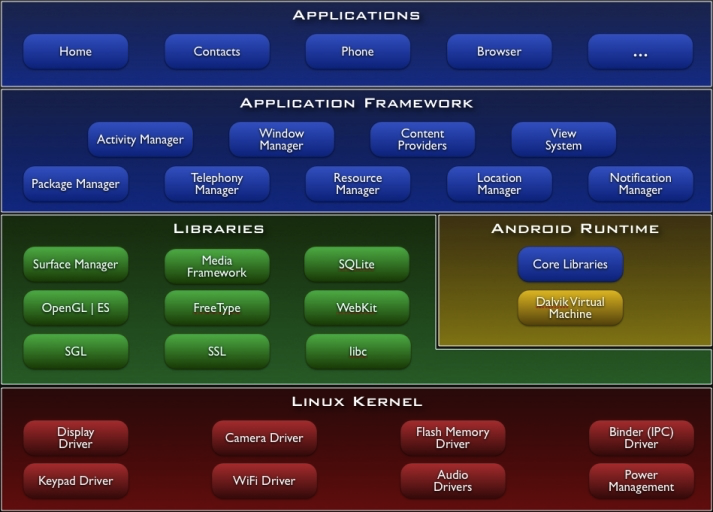
\includegraphics[scale=0.35]{system-architecture}
\end{frame}

\begin{frame}
\frametitle{안드로이드 프레임워크 개요 수정본(From kandroid)}
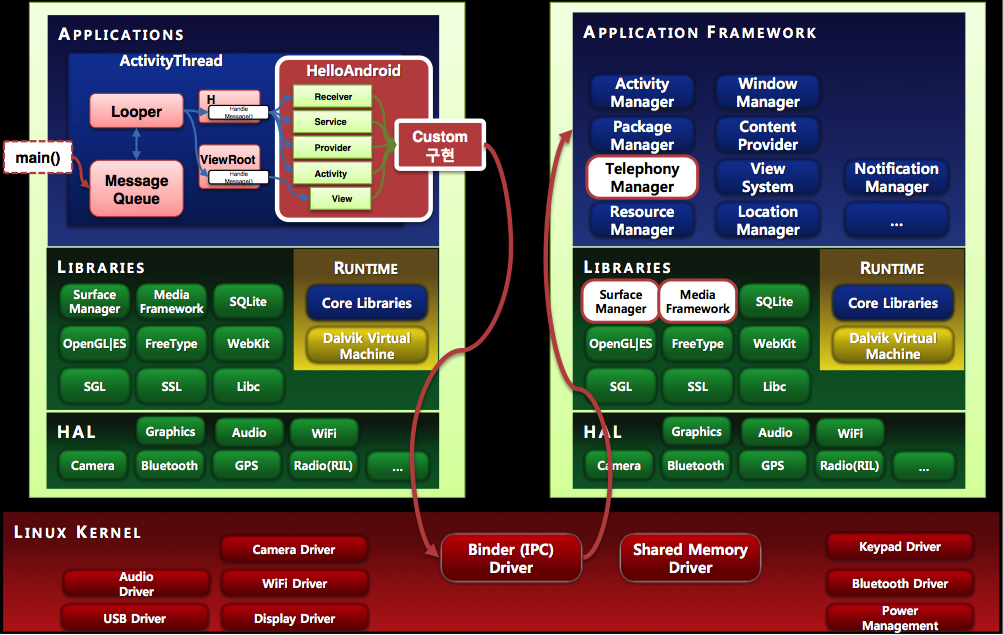
\includegraphics[scale=0.3]{kandroid-framework}
\end{frame}

\begin{frame}
\frametitle{안드로이드 프로세스 보기}
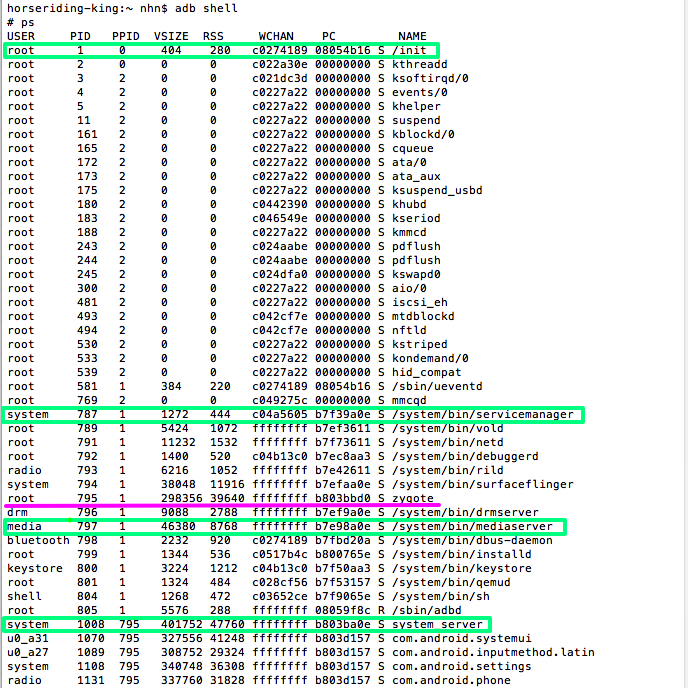
\includegraphics[scale=0.3]{ps}
\end{frame}

\begin{frame}
\frametitle{Binder(From 인사이드 안드로이드)}
\begin{itemize}
\item 안드로이드 프로세스는 고유한 가상공간에서 실행되는데, 3G의 사용자 공간과 1G의 커널 공간으로 나뉜다. 사용자 코드와 관련 라이브러리는 사용자 공간의 코드 영역, 데이터 영역, 스택 영역에서 동작한다.
\item 프로세스간 통신은 모든 프로세스가 공유하는 커널 공간을 이용한다. Binder IPC Driver는 프로세스간 메시지를 주고 받는 IPC를 지원한다. 
\item http://helloworld.naver.com/helloworld/47656
\end{itemize}
\end{frame}

\begin{frame}
스레드는 언제 어떻게 사용할까?
\end{frame}

\begin{frame}
\frametitle{군더더기 코드들}
\begin{itemize}
\item AsyncTask를 Service나 BroadcastReceiver에서도 사용한다. 
\item 스레드 작업이 예를 들어 2초면 끝나겠거니 예상하고서, sleep을 주고서 다음 작업을 진행한다.
\item 시간이 걸리면서, 앱의 기반이 되는 데이터를 Application.onCreate에서 작업 스레드를 만들어 처리하게 한다.(예를 들어 캘린더앱에서 휴일 정보)
\end{itemize}
\end{frame}

\begin{frame}
\frametitle{ThreadPoolExecutor}
\begin{itemize}
\item 스레드풀은 대기 상태의 스레드를 유지해서 task 실행 오버헤드를 줄임으로써 많은 갯수의 비동기 작업을 실행할 때 퍼포먼스를 향상 시킨다. 
\item 컴포넌트에 작업이 계속 들어온다면 스레드풀 사용을 고려해보자. AsyncTask도 내부적으로 스레드풀을 사용하고 있다.
\end{itemize}
\end{frame}

\begin{frame}
\frametitle{ThreadPoolExecutor 생성자}
ThreadPoolExecutor(int corePoolSize, int maximumPoolSize, long keepAliveTime, TimeUnit unit, BlockingQueue$<$Runnable$>$ workQueue, RejectedExecutionHandler handler)
\begin{itemize}
\item pool의 스레드 갯수가 coreSize보다 커진다면, 초과하는 갯수만큼의 작업은 끝나고 나서는 스레드를 유지할 필요는 없다. keepAliveTime과 unit은 이때 바로 제거하지 않고 대기하는 시간이다. 보통 unit에는 TimeUnit.MINUITES나 TimeUnit.SECONDS 정도를 사용한다. 
\item pool에서는 corePoolSize만큼 유지하려 하고, 추가로 요청이 들어오면 workQueue에 쌓아놓는다. 이 workQueue 갯수 제한이 넘으면 pool의 스레드 갯수를 늘려야만 한다. 
\end{itemize}
\end{frame}

\begin{frame}
\frametitle{RejectedHandler}
ThreadPoolExecutor가 shutdown되거나, 최대 스레드갯수와 workQueue 용량을 넘어갔을 때는 task가 거부된다. 거부되는 방식을 정하는 것이 RejectedExecutionHandler이고, 미리 정의된 hanlder가 4개 있다.
\begin{itemize}
\item ThreadPoolExecutor.AbortPolicy : 디폴트 handler로 RejectedExecutionException 런타임 예외를 발생시킨다.
\item ThreadPoolExecutor.CallerRunsPolicy : 요청 task가 호출하는 스레드에서 바로 실행된다. 
\item ThreadPoolExecutor.DiscardPolicy : 요청 task가 조용히 제거된다.
\item ThreadPoolExecutor.DiscardOldestPolicy : workQueue에 맨 위에 있는 오래된 task를 제거한다.
\end{itemize}

\end{frame}

\begin{frame}
\frametitle{ScheduledThreadPoolExecutor}
\begin{itemize}
\item 지연/반복 작업에 대해서는 ScheduledThreadPoolExecutor 사용을 고려하자.
\item Handler를 이용해서도 지연/반복 작업을 할 수도 있다고 했는데, 화면 갱신이라면 Handler를 쓰는 게 적절하지만, 네트웍 통신이나 DB 작업 같은 것이 지연/반복 실행되는 경우를 예로 들 수 있다.
\item Timer를 쓰지 말고 ScheduledThreadPoolExecutor를 사용하자. Timer는 실시간 task 스케줄링을 보장하지 않고(스레드를 하나만 생성해서 사용하기 때문에 앞에 먼저 실행되는 작업 때문에 예정 시간에 맞지 않게 실행될 수 있다), 여러 스레드가 동기화 없이 하나의 타이머를 공유할 수 있는 문제가 있다.
\end{itemize}
\end{frame}

\begin{frame}
\frametitle{프로세스의 우선순위}
\Fontvi
http://developer.android.com/guide/components/processes-and-threads.html
\begin{enumerate}
\item Foreground process: 사용자와 interact하는 Activity를 가지고 있거나, 그런 Activity에 bound된 Service를 가지고 있거나, startForeground를 호출한 foreground Service를 가지고 있거나, Service의 생명주기(onCreate, onStart, onStartCommand, onDestroy)를 실행중인 Service를 가지고 있거나, onReceive를 실행하는 BroadcastReceiver를 가지고 있는 경우이다.
메모리가 부족할 때에도 가장 마지막까지 남아있을 수 있는 process들이다.
\item Visible process: foreground 컴포넌트를 가지고 있지는 않지만, 사용자가 보는 화면에 아직 영향이 있다. Activity로 치면 onPause까지 탔지만 visible 상태인 것이다.(다이얼로그 테마나 투명한 Activity가 가렸을 때)
visible Activity에 bound된 Service를 가진 경우도 해당한다. 
\item Service process: startService로 실행했지만, 위의 카테고리에는 들어가지 않는 Service를 가진 경우이다. 이런 것들은 사용자가 지금 보고 있는 것과 직접적인 연관은 없다. Service에서 작업 스레드를 실행하는 중이라면, 생명주기를 타고 있는 것은 아니다.
\item Empty process: 사용자가 Back 키로 종료를 하고 활성화된 컴포넌트가 없다면,  empty process가 된다. 이런 프로세스를 메모리에 갖고 있는 이유는 다음에 컴포넌트를 띄울때 빠르게 띄우려고 하는 cache 용도일 뿐이다. 가장 우선순위가 낮아서 리소스가 부족하면 가장 먼저 kill 대상이 된다.
\end{enumerate}
\end{frame}

\begin{frame}
\frametitle{스레드를 안정적으로 돌리려면}
\begin{itemize}
\item 앱이 스레드를 마치기 전에 Back으로 나가서 한참 다른 앱을 사용하느라고 관심을 안 준다면, 프로세스가 kill될 수 있다. 이 스레드가 프로세스 우선순위상 더 진행을 하지 못하고 제거되는 운명에 처할 가능성이 있는데, 오래 걸리는 작업의 안정성을 보장할 수가 없다.
\item Service 상에서 스레드를 시작한다. 프로세스 우선순위상 제거될 가능성이 줄어들고, 프로세스가 kill되어도 Service는 onStartCommand 리턴값에 따라 재시작할 수 있다.
\end{itemize}
\end{frame}

\begin{frame}
\frametitle{Service는(1)}
\begin{itemize}
\item 혹자는 Service는 Thread를 안정적으로 돌리기 위한 컴포넌트라고 얘기하기도 한다. 실제 개발에 상당히 유용한 얘기이고, Service에 대한 이해에도 많은 도움을 준다.\\
\item Service를 얘기할 때면, 자주 나오는 얘기가 백그라운드 상에서 실행되는 컴포넌트라고 한다. Activity 처럼 눈에 보이는 visible 컴포넌트가 아니라는 의미로 백그라운드인 것으로, Main UI 스레드가 아닌 별도의 스레드에서 실행하는 것으로 착각해서는 안 된다.\\
\end{itemize}
\end{frame}

\begin{frame}
\frametitle{Service는(2)}
\begin{itemize}
\item Service 역시 UI 스레드상에서 실행되므로, intensive \& blocking 작업을 한다면, Activity에서 UI를 처리하지 못하는 상황이 생길 수 있으므로, Service에서 별도의 스레드를 생성해야 하는 경우가 일반적이다.\\
\item Service는 해당 앱에서 하나의 인스턴스밖에 생기지 않는다. 따라서 우리는 일부러 Singleton 객체를 만들고 그 안에서 Thread를 돌리는 일 같은 것은 할 필요가 없다. 훨씬 안정적으로 동작하는 컴포넌트를 활용하기만 하면 된다.
\end{itemize}
\end{frame}

\begin{frame}
\frametitle{Service를 시작하는 방법}
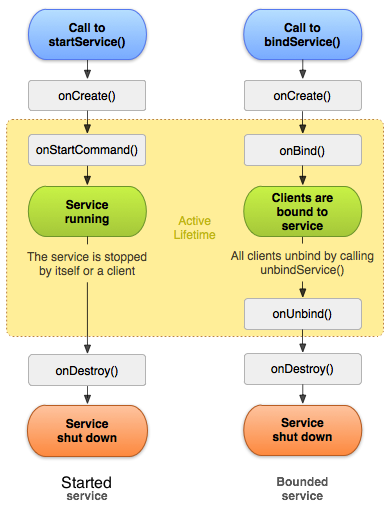
\includegraphics[scale=0.4]{service-lifecycle}
\end{frame}

\begin{frame}
\frametitle{Started Service}
\begin{itemize}
\item 명령을 던져놓고 알아서 돌도록 하는 작업에 적합하다.
\item onCreate는 아직 생성되지 않은 경우에만 호출하고, 그 이후에는 onStartCommand만을 호출한다.
\item startService하는 시점에 시작하는 것이 아니고, 메시지큐에 Service를 시작하도록 들어가고 메인 스레드를 쓸 수 있는 시점에 시작된다.
\item 표준 패턴은 onStartCommand에서 별도 작업 스레드를 생성해서 시작하는 것이다.
\end{itemize}
\end{frame}

\begin{frame}
\frametitle{onStartCommand 리턴값의 의미}
\Fontvi
디폴트 값은 START\_STICKY이다.
\begin{enumerate}
\item START\_NOT\_STICKY: started 되고서(onStartedCommand가 리턴된 상태) kill 되면, 재생성하지 않는다. 명시적으로 start 할 때만 의미가 있는 작업에 사용한다. 예를 들어 화면에서 뉴스를 가져다놓으라고 명령을 줄 수가 있는데, 메모리 이슈로 인해 서비스가 kill되었다면, 다시 명령을 주기를 기다려서 최신 뉴스를 가져다 주는 것이 나을 수 있다.
\item START\_STICKY: 재시작시에 다시 onStartCommand를 호출하는데, 이때 Intent 매개변수가 null로 전달된다. startService할 때 Intent에 값을 전달하고, 이 값을 startCommand에서 사용할 시에는, NullPointer 발생 가능성이 있다. start 시키는 쪽에서 전달한 값을 사용하지 않고, 내부적인 상태만을 가지는 서비스에 적합하다.\\
예) 서버 API 에 접근해서 날씨 정보를 가져와서 업데이트 하는 것과 같은 지속적인 데이터 Sync 작업
\item START\_REDELIVER\_INTENT:  재시작시에 onStartCommand에 Intent를 다시 전달하여 호출한다. 어떻게든 해당 파라미터를 가지고 실행시켜야 하는 Service가 이에 해당한다. 쇼핑몰 앱에서 어느 회사의 상품 정보를 API를 통해서 가져온 후 DB에 저장해야 한다면, 이런 경우에 쓸 수 있다.\\
\end{enumerate}
\end{frame}

\begin{frame}
\frametitle{불필요한 재시작 방지}
\begin{itemize}
\item Service는 할 일은 다 끝났는데 불필요하게 메모리를 차지하고 있고, started 상태로 남아있고, 어느 순간에 메모리 이슈로 Service가 kill되면 리턴 상수에 따라 의도치 않게 재시작하는 일이 생길 수 있다.
\item 이 재시작은 조금 양상이 다르다. 곧바로 재시작하는 것이 아니라, 다음에 startService를 할 때 앞에 먼저 처리해야 하는 것처럼 기존의 것에서 한번 onStartCommand가 먼저 실행된다.
\item Service안에서 작업이 끝났으면 스레드 안에서 명시적으로 stopSelf를 호출한다.
\end{itemize}
\end{frame}

\begin{frame}
\frametitle{멀티 스레드 이슈}
\begin{itemize}
\item 여러 곳에서 startService를 호출할 수 있다. 어차피 onCreate나 onStartCommand는 메인 스레드에서 실행되므로 상관이 없지만, onStartCommand안에서 실행한 작업 스레드들은 동시에 여러 개가 돌고 있을 수 있기 때문에 값을 잘못 공유하면 문제가 발생할 수 있다.
\end{itemize}
\end{frame}

\begin{frame}
\frametitle{IntentService}
\begin{itemize}
\item 일반적인 앱에서 멀티스레딩이 필요한 경우가 많지는 않다. 동시에 여러 요청을 처리할 필요가 없다면, IntentService를 활용하자.
IntentService는 내부적으로 별도의 스레드를 두고 전달된 Intent를 순차적으로 처리한다.\\
IntentService에서는 별도 스레드에서 실행되는 내용인 onHandleIntent(Intent) 메소드만 구현하면 된다.
\item IntentService에서 내부적으로 구현한 onStartCommand() 메소드는 기본 리턴값은 START\_NOT\_STICKY이다.
\end{itemize}
\end{frame}

\begin{frame}[fragile]
\frametitle{Service 중복 실행 방지}
여러 곳에서 startService를 하는 경우, 모두 실행하지 않고 이미 시작되었으면 나머지는 skip 하고자 할 때가 있다.\\
소스 코드는 교재 참고
\end{frame}

\begin{frame}
\frametitle{Bounded Service}
\begin{itemize}
\item Remote Binding과 Local Binding이 있다.
\item Binding 된 이후에 메소드 호출은 Client/Server 관계로 Blocking이 된다.
\item Local Binding은 큰 의미를 두지 말자. Local Bounded Service를 만들지 않고 일반 클래스로도 가능하다. 싱글톤을 만들어주는 정도로만 보면 된다.
\end{itemize}
\end{frame}

\begin{frame}
\frametitle{Remote Binding(1)}
\begin{itemize}
\item 인터페이스를 만드는 형태로 aidl 파일을 만들면 gen에 Binder 통신을 하는  자바 소스가 생성된다.(교재 참고)
\item 생성 코드에서 클라이언트는 Proxy, 서버는 Stub을 사용하며 Service에서는 Stub의  구현체를 만든다. 이 구현체에서는 결국 aidl에 정의된 메소드를 작성한다.
\item 동일한 프로세스에 있다면, Binder를 거치지 않고 직접 호출한다.
\item 리모트인 경우 Service가 속한 프로세스의 Binder 스레드풀(DDMS에서 스레드명을 보면 Binder\_1, Binder\_2 이런 이름으로 나온다. 최대 15개까지 만들어진다.)에서 실행된다.
\end{itemize}
\end{frame}

\begin{frame}
\frametitle{Remote Binding(2)}
\begin{itemize}
\item bindService는 Binding 결과를 비동기로 받기 때문에, Callback으로 사용할 ServiceConnection 인스턴스를 전달한다.(교재 참고)
\item Service의 onBind에서 리턴하는 인스턴스가 실제 클라이언트에서 사용하는 것이다. Service는 매개체가 되는 것 뿐이다.
\item Remote와 연결이 끊어질 수도 있기 때문에 Service를 호출할 때에는 유효한지 먼저 체크한다.(교재 참고)
\end{itemize}
\end{frame}

\begin{frame}
\frametitle{aidl에서 쓸 수 있는 데이터 타입은 제한되어 있다.}
Marshaling/Unmarshaling을 해야 하기 때문이다.\\
기본적으로 지원하는 타입을 보자. 
\begin{enumerate}
\item primitive type(int, long, char, boolean 등)
\item String
\item List: 구체 클래스인 ArrayList 같은 건 쓸 수 없다. generic도 약간은 쓸 수 있다. List$<$String$>$, List$<$List$>$ 같은 건 되지만, List$<$?$>$, List$<$List$<$Sting$>>$ 같은 건 안 된다.
\item Map: 역시 구체 클래스인 HashMap 같은 건 쓸 수 없다. generic은 지원하지 않는다.
\end{enumerate}

우리가 만드는 클래스들은 어떻게 지원할까 하면 바로 Parcelable 인터페이스를 구현하면 된다. Parcelable로 만들지 않으면, aidl에 import도 되지 않는다.(aidl 파일과 동일한 패키지에 있는 클래스도 import 해줘야 한다.)\\
\end{frame}

\begin{frame}
\frametitle{Binding의 특성(1)}
\begin{itemize}
\item bindService를 하면 Service와 엮이는 클라이언트가 하나씩 늘어난다고 보면 된다. 이렇게 엮인 클라이언트가 남아 있다면 stopService를 해도 종료가 되지 않는다. 모든 클라이언트가 unbindService 메소드를 호출해서 Service와의 관계가 정리되어야만 한다.
\item onServiceDisconnected는 Service에 문제가 생겼을 때(주로 crash 되거나 kill 되었을때) 호출되는 것이다. Service Binding은 유효한 상태이고, 다음에 running 상태가 되면 onServiceConnected가 알아서 다시 호출된다.(어떤 책에서는 ServiceConnection의 onServiceDisconnected가 Service에서 onUnbind 된 이후에 호출된다고 잘못 나오기도 한다. 주의하자!)
\end{itemize}
\end{frame}

\begin{frame}
\frametitle{Binding의 특성(2)}
\begin{itemize}
\item Activity에서 Bounded Service를 사용할 때는, onStart와 onStop에서 bindService와 unbindService를 각각 호출하는 것을 권장하고 있다. unbindService시 붙어있는 클라이언트 수가 0가 되면 서비스는 종료될 수 있음을 생각해보자. onResume/onPause는 빈번하게 transition이 일어나는데(전원버튼 누르기, 홈 key로 이동하기 등), onPause를 통해 Service가 종료되었다가 onResume에서 다시 시작해야 될 수 있다. 종료된 Service라면 다시 생성하는 비용이 들게 되는데, 빈번한 transition에서는 적합하지 않다. 
\item 클라이언트에서 메소드를 호출하면 Service에서 결과를 리턴해주어야 하는데, Service에서도 작업이 오래 걸린다면, 스레드로 빼는 것을 고려할 수 있다. 스레드의 작업이 다 되었을때 Broadcast를 전달해서, 다시 Client한테 가져가라고 요청할 수도 있고, Callback을 Service에 전달해서 결과를 받는 방법도 있다. Callback도 Binder 통신을 해야 하므로 aidl로 작성해야 한다.
\end{itemize}
\end{frame}

\begin{frame}
Activity에서 this, getBaseContext(), getApplicationContext()는 어떻게 다른가?
\end{frame}

\begin{frame}
\frametitle{Context}
\begin{itemize}
\item Interface to global information about an application environment.
\item 앱을 개발하면 항상 만나게 되는 클래스이다.
\item Context 클래스가 없으면 Activity를 시작할 수도, Broadcast를 발생시킬 수도, Service를 실행할 수도 없다. 리소스에 접근하려 할 때도 Context가 있는 상태에서만 가능하다.\\
Context를 통해서 여러 컴포넌트가 연결돼있고, Context가 애플리케이션의 알아야 하는 시작점이라고 할 수 있다.
\end{itemize}
\end{frame}

\begin{frame}
\frametitle{Context의 상속(1)}
\begin{itemize}
\item Context는 기본적으로 추상 클래스인데, 메소드 구현이 거의 없고, 상수 정의와 추상 메소드들로 이루어져 있다. 그럼 이것을 상속한 것들은 무엇인가. 주요한 것들을 얘기하자면, 직접 상속한 것은 ContextWrapper이고, ContextWrapper를 상속한 Activity, Service, Application이 있다.
\item ContextWrapper 클래스에는 그 이름처럼 ContextWrapper(Context base) 생성자를 갖고 있다.\\
바로 이 생성자에 들어가는 것이 실제 Context의 수많은 메소드들을 직접 구현한 ContextImpl 클래스이다.
ContextWrapper의 수많은 메소드는 실제로 base의 메소드를 그대로 호출하는 것 밖에 하지 않는 다.
\end{itemize}
\end{frame}

\begin{frame}
\frametitle{Context의 상속(2)}
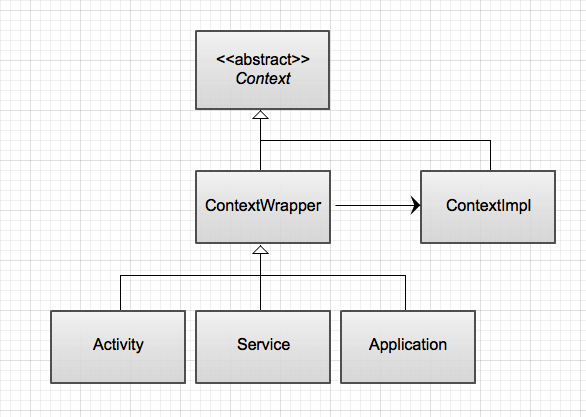
\includegraphics[scale=0.3]{context}
\end{frame}

\begin{frame}
\frametitle{ContextImpl}
\begin{itemize}
\item 컴포넌트가 생성될 때마다 새로 생성해서 ContextWrapper에 전달된다.
\item static intializer block에서, 시스템 서비스 매핑을 한다.
\item Activity, Service, Application은 새로 생성한 ContexImpl을 각각 Wrapping 하고, getBaseContext()로 ContextImpl을 가져온다.
\end{itemize}
\end{frame}

\begin{frame}
\frametitle{Context 가져오기}
\begin{itemize}
\item Context.getApplicationContext()는 Application 인스턴스를 가져온다. 
\item BroadcastReceiver, ContentProvider에 전달되는 Context는 Application 인스턴스이다.
\item Activity에서 setContentView 이후에 findViewById 한 View에서 getContext()를 하면 Activity 자신이 리턴된다.
\end{itemize}
\end{frame}

\begin{frame}
\frametitle{Activity를 사용할 것인가?}
\begin{itemize}
\item Activity가 AndroidManifest.xml에 추가하면 되지만, 많으면 유지하기가 힘들게 되므로, Activity는 불필요하게 많이 만들지 말자.
\item 내부에 UI 액션이 많고 로직이 많다면 우선 Activity를 고려하고, 
위에 팝업 형식으로 뜬다면, 커스텀 뷰 다이얼로그나 DialogFragment, PopupWindow로 대체를 고려한다.
'로딩중'이라고 전체를 덮는 반투명 화면은 어떨까? 이런 것도 Activity보다는 DialogFragment가 적절하다.
\item 기준은 단순하게 하자. 독립적인 하나의 화면이라고 하면 Activity가 맞고, 종속적인 화면이라고 보이면 다른 것을 쓸 수 있는지 생각해 보자.
\end{itemize}
\end{frame}

\begin{frame}
\frametitle{Activity 생명주기}
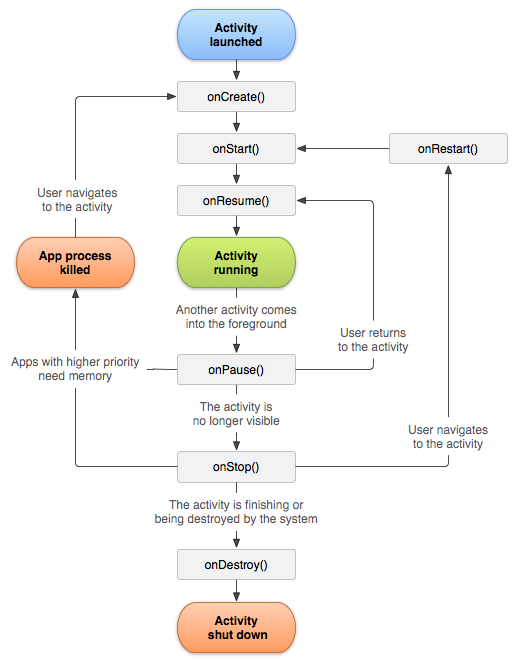
\includegraphics[scale=0.3]{activity-lifecycle}
\end{frame}

\begin{frame}
\frametitle{케이스별 생명주기 메소드 호출(1)}
\begin{itemize}
\item \fbox{\bfseries 시작될때/방향 바뀔때}
onCreate $\rightarrow$ onStart $\rightarrow$ onResume\\

\item \fbox{\bfseries 다른 Activity가 위에 뜰 때/홈 키}
onPause $\rightarrow$ onStop\\
% 홈 키 확인 필요하다.
\item \fbox{\bfseries Back으로 나갈때}
onPause $\rightarrow$ onStop $\rightarrow$ onDestroy\\

\item \fbox{\bfseries Back 키로 돌아올때/Home 키로 갔다가 돌아올때}
onRestart $\rightarrow$ onStart $\rightarrow$ onResume\\

\item \fbox{\bfseries 전원키 꺼질 때/Dialog Theme를 가진 Actitivity가 위에 뜰때}\newline \fbox{\bfseries 투명 액티비티가 뜰때}
onPause
\end{itemize}
\end{frame}

\begin{frame}
\frametitle{케이스별 생명주기 메소드 호출(2)}
\begin{itemize}
\item onCreate에서 finish를 호출하면 다른 생명주기 메소드를 거치지 않고, 곧 바로 onDestroy를 탄다.
\item onActivityResult는 onResume보다 먼저 실행된다.
\end{itemize}
\end{frame}

\begin{frame}
\frametitle{Activity간 생명주기 메소드 실행}
\begin{block}{Activity A에서 Activity B를 start할 때}
\begin{enumerate}
\item Activity A 는 onPause 메소드를 실행한다.
\item Activity B 는 onCreate, onStart, onResume 메소드를 실행하고, 포커스를 갖는다.
\item Activity A는 onStop 메소드를 실행한다.
\end{enumerate}
\end{block}
\begin{block}{반대로 Activity B가 닫힐 때}
\begin{enumerate}
\item Activity B는 onPause 메소드를 실행한다.
\item Activity A는 onRestart, onStart, onResume 메소드를 실행한다.
\item Activity B는 onStop, onDestroy 메소드를 실행한다.
\end{enumerate}
\end{block}
\end{frame}

\begin{frame}
\frametitle{생명주기 메소드 실행시 주의사항}
\begin{itemize}
\item 리소스 관련해서 생명주기 상에서 대칭을 맞춘다.(onCreate-onDestroy, onResume-onPause, onStart-onStop)
\item super.onXXX 호출 순서를 일정하게 한다. 시작할 때는 super를 먼저 하고 종료하는 쪽에서는 super를 나중에 한다.
\item finish() 메소드 호출하고 다른 일을 하지 말자. 가능하면 바로 return 한다. 
\item onXXX 메소드는 직접 호출하지 말자.
\end{itemize}
\end{frame}

\begin{frame}
\frametitle{Activity Task 확인하기}
\begin{itemize}
\item 눈으로만 동작 확인해서는 원하는 동작인지 확인이 어렵다.
\item adb shell dumpsys activity activities를 통해서 Task을 확인하자. activities 대신 a만 써도 된다.
\end{itemize}
\end{frame}

\begin{frame}
\frametitle{Activity에 Task 속성 부여}
\begin{itemize}
\item Callee 속성 부여는 AndroidManifest.xml의 Activity 선언에 android:launchMode로 한다.
\item Caller 속성 부여는 Intent의 Flags에 전달한다. Flags에는 가능한 최소한의 Flag만 전달해야 한다.
\end{itemize}
\end{frame}


\begin{frame}
\frametitle{Activity에서 이런 거 하지 말자}
\begin{itemize}
\item findViewById 해서 불필요한 Casting은 하지 말자. 
\item 상속 구조를 깊게 하지 말자.
\item Activity에서 너무 많은 Listener 인터페이스를 구현하지 말자.
\end{itemize}
\end{frame}

\begin{frame}
\frametitle{Activity에서 이렇게 해보자.}
\begin{itemize}
\item static 메소드로 startActivity를 실행한다.
\item 여러 위젯이 있을 때 동일한 위젯끼리 모아놓는다.
\item 상수나 멤버 변수는 쓰이는 위치 근처에 선언한다.
\end{itemize}
\end{frame}

\begin{frame}
\frametitle{BroadcastReceiver}
\begin{itemize}
\item 시스템이나 앱의 이벤트를 Broadcast 형태로 전달하면, 여러 Receiver에서 받아서 처리하는 형태로, Observer 패턴을 안드로이드에서 적용한 방식이다.
\item 이벤트가 발생했을때 이벤트에 대응하는 작업으로 Activity나 Service를 시작하는 경우가 많다.
\end{itemize}
\end{frame}

\begin{frame}
\frametitle{BroadcastReceiver 유의할 점}
\begin{itemize}
\item Thread를 onReceiver 메소드 안에서 실행하면 스레드의 정상 실행을 보장할 수 없다. AsyncTask 역시 마찬가지다.
\item 메인 스레드에서 onReceive가 실행되므로, 한 이벤트에 대해서 앱에서 많은 BroadcastReceiver가 받게 되어 있다면, UI 동작에 심각한 문제를 만들 수 있다.
\end{itemize}
\end{frame}


\begin{frame}
\frametitle{Application의 사용 용도}
\begin{itemize}
\item Application.onCreate에서 앱의 초기화 작업을 한다. 가능한한 빨리 끝나야만 한다. 그렇지 않으면 메인 Activity 실행시 검은 화면을 보게 된다.
\item 앱 전체적으로 사용하는 Single 인스턴스를 공유한다. Singleton을 따로 만들지 않아도 된다.
\item 앱 에서 컴포넌트간에 데이터를 공유한다.
\item 항상 떠있는 컴포넌트이기 때문에, Context를 참조해야 할 때 Application을 사용하기도 한다.(억지로 쓰는 방법)
\end{itemize}
\end{frame}


\begin{frame}
\frametitle{프로세스 분리}
\begin{itemize}
\item 주로 메모리 이슈 때문에 프로세스 분리를 하고, Activity/Service/ContentProvider/BroadcastReceiver 모두 프로세스 분리가 가능하다.
\item 동일 패키지에서 생성된 별도 프로세스는 pid(process id)는 다르지만, 동일한 uid(user id)를 가지고 동일하게 파일과 리소스에 접근할 수 있다.
\item 프로세스 분리가 되었을때, Application은 각 프로세스마다 새로 시작된다.
\end{itemize}
\end{frame}

\begin{frame}
\frametitle{프로세스 분리시 주의할 점}
\begin{itemize}
\item 당연한 얘기지만 메모리 공유가 안 된다. 개발하는 중에는, 별 차이가 없어서 잊기 쉽다.
\item 분리된 프로세스에서는 SharedPreferences 가져올 때 mode가 중요하다. Honeycomb 이상에서는 Context.MODE\_MULTI\_PROCESS를 사용해야 한다.
\end{itemize}
\end{frame}

\end{document}